\section{Pytorch 张量操作}
\subsection{创建 Tensor}
\subsubsection{从 numpy 导入}
\begin{lstlisting}
  torch.from_numpy(numpy.array)
\end{lstlisting}

\subsubsection{从 list 导入}
\begin{lstlisting}
  torch.tensor('list')
\end{lstlisting}

\subsubsection{未初始化}
\begin{lstlisting}
  torch.empty(shape_no_list)
  torch.Tensor(shape_no_list)
  torch.IntTensor(shape_no_list)
  torch.FloatTensor(shape_no_list)
\end{lstlisting}

\subsubsection{设置 Tensor 默认类型}
\begin{lstlisting}
  torch.set_default_tensor_type(torch.FloatTensor/DoubleTensor)
\end{lstlisting}

\subsubsection{随机初始化}
\begin{lstlisting}
  rand(shape)
  randint('min,max',[shape]) '\#'['min,max')
  rand_like(tensor)
  randn(shape)  '\#'data - N(0,1)
\end{lstlisting}
%torch.normal(mean=torch.full([10], 0), std=torch.arange(1, 0, -0.1))

\subsubsection{初始化为同一个数}
\begin{lstlisting}
  torch.full([shape],number)
\end{lstlisting}

\subsubsection{生成递增递减序列}
\begin{lstlisting}
  torch.arange('min', 'max', step)      '\#'['min, max')   'int'
  torch.linspace('min', 'max', steps)      '\#'['min, max']   steps=numbers   'float'
  torch.logspace('min', 'max', steps)    '\#'['min, max']   step^n'
\end{lstlisting}

\subsubsection{ones/zeros/eyes/*\_like}
\begin{lstlisting}
  torch.ones(shape)
  torch.zeros(shape)
  torch.eye(shape)
  torch.*_like(tensor)
\end{lstlisting}

\subsubsection{生成随机种子}
\begin{lstlisting}
  torch.randperm('int')
\end{lstlisting}
~\\
~\\
~\\
~\\
~\\





\subsection{索引和切片}
\subsubsection{简单索引}
\begin{lstlisting}
  a = torch.rand(10,3,28,28)
  a[0]    '\#''第0张照片'
  a[0,0]    '\#''第0张照片的第0个通道'
  a[0,0,0]    '\#''第0张照片的第0个通道的第0行像素 dim为1'
  a[0,0,0,0]    '\#''第0张照片的第0个通道的第0行的第0个像素 dim为0'
\end{lstlisting}

\subsubsection{利用切片选取连续索引}
\begin{lstlisting}
  a = torch.rand(10,3,28,28)
  a[:2]   '\#''取前两张图片'
  a[-2:]    '\#''取后两张图片'
  a[:2,:1]    '\#''取前两张图片的第一个通道'
  a[-2:,-2:]     '\#''取后两张图片的后两个通道'
\end{lstlisting}

\subsubsection{利用切片选取间隔索引}
\begin{lstlisting}
  a[:,:,0:28:2,0:28:2]      '\#''取全部图片的全部通道的长宽均间隔采样'
\end{lstlisting}

\subsubsection{选取不规则索引}
\begin{lstlisting}
  a[2][1][18][26]   '\#''取第2张图片的第1通道的第18行26列的像素值,标量'
  a.index_select(dim,tensor)   '\#''第一个参数表示维度,第二个是tensor值'
  a.index_select(0,torch.tensor([0, 3, 3]))   '\#''选择第0第3第3张图片'
  a.index_select(1,torch.tensor([0,2]))   '\#''选择四张图片的第0和第2的通道'
  a.index_select(2,torch.arange(0,8))   '\#''选择四张图片每个通道的前8所有列的像素'
\end{lstlisting}

\subsubsection{使用符号 ... 推测维度}
\begin{lstlisting}
  a[...].shape
  a[:3,...].shape
  a[:,1,...].shape
  a[...,:10].shape
  a[0,...,::2].shape    '\#''间隔采样 ::'
\end{lstlisting}

\subsubsection{依据掩码的位置信息索引}
\begin{lstlisting}
  x = torch.randn(3,3)
  mask = x.ge(0.5)    '\#''>=0.5的位置信息'
  torch.masked_select(x,mask)    '\#''得到所有>=0.5的tensor值'
\end{lstlisting}

\subsubsection{打平索引}
\begin{lstlisting}
src = torch.tensor([[1,2,3], [4,5,6]])
torch.take(src, torch.tensor([0,2,5])).shape          '\#torch.Size([3])'
\end{lstlisting}
~\\
~\\
~\\
~\\

\subsection{Tensor 维度变换}
\subsubsection{重塑维度-reshape/view}
\begin{lstlisting}
tensor.view(a,b,c,...)
tensor.reshape(a,b,c,...)
\end{lstlisting}

\subsubsection{删减增加维度-squeeze/unsqueeze}
\begin{figure}[!h]
  \centering
  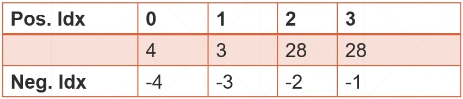
\includegraphics[width=1\textwidth]{unsqueeze.png}
\end{figure}
\begin{lstlisting}
  a = torch.rand(4, 3, 28, 28)
  a.unsqueeze(0).shape     '\#[1, 4, 1, 28, 28] 0维度前面插入一个维度'
  a.unsqueeze(-1).shape     '\#[4, 1, 28, 28, 1] 在最后一个维度后面插入一个维度'
  a = torch.rand(1, 32, 1, 1)
  a.squeeze().shape     '\#torch.Size([32]) 尽可能多的删减维度'
  a.squeeze(0).shape     '\#torch.Size([32, 1, 1])'
  a.squeeze(-2).shape     '\#torch.Size([1, 32, 1])'
\end{lstlisting}

\subsubsection{单次多次交换维度-transpose/permute}
\begin{lstlisting}
a = torch.randn(3,4)
a.t()     '只能适用于二维转置'
\end{lstlisting}
\begin{lstlisting}
  a = torch.randn(4, 3, 28, 28)    '记录维度信息否则污染数据'
  b = a.transpose(1,3).reshape(4, 3*28*28).reshape(4, 3, 28, 28)    '数据污染'
  c = a.transpose(1,3).reshape(4, 3*28*28).reshape(4, 28, 28, 3)
  .transpose(1,3)
  torch.all(torch.eq(a, b))     '\#tensor(0, dtype=torch.uint8)'
  torch.all(torch.eq(a, c))     '\#tensor(1, dtype=torch.uint8)'
\end{lstlisting}
\begin{lstlisting}
  'transpose 只能做单次交换 但 permute 可以做多次交换'
  a = torch.randn(4, 3, 28, 32)     '目标(4, 28, 32, 3)'
  a.transpose(1, 3).transpose(1, 2).shape     '\#torch.Size([4, 28, 32, 3])'
  a.permute(0, 2, 3, 1).shape     '\#torch.Size([4, 28, 32, 3])'
\end{lstlisting}

\subsubsection{维度扩展-expand/repeat}
\begin{lstlisting}
  'rexpand  表示扩展到的维度   内存无关'
  tensor.expand(a,b,c,d)
  'repeat  表示复制次数    内存相关'
  tensor.repeat(a,b,c,d)
\end{lstlisting}




\newpage
\section{Pytorch 张量高阶操作}
\subsection{Broadcasting}
\begin{figure}[!h]
  \centering
  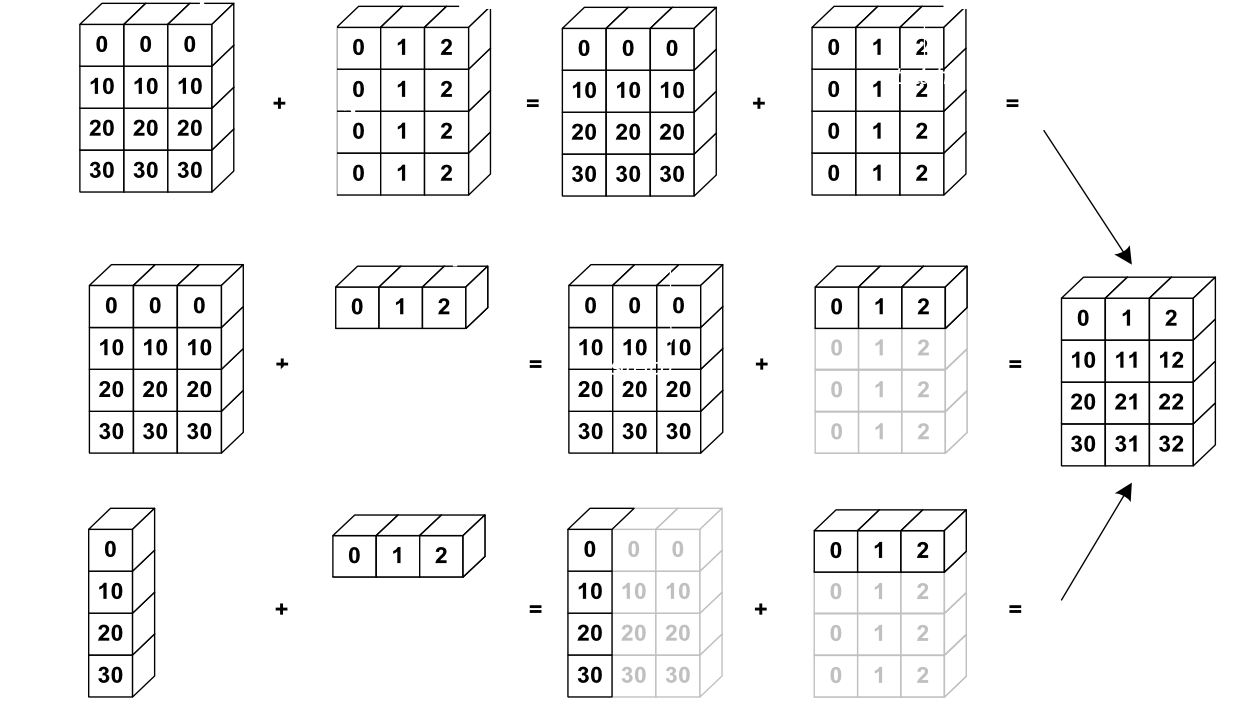
\includegraphics[width=0.95\textwidth]{broadcasting.png}
\end{figure}
~\\
~\\
~\\
~\\
~\\

\subsection{Tensor 分割与合并}
\subsubsection{合并不增加维度-cat}
\begin{lstlisting}
a = torch.rand(4, 32, 8) '\#[classes, students, scores]'
b = torch.rand(5, 32, 8)   'cat维度可以不同'
torch.cat([a, b],dim=0).shape '\#torch.Size([9, 32, 8])'
\end{lstlisting}

\subsubsection{合并增加维度-stack}
\begin{lstlisting}
a = torch.rand(32, 8) '\#[students, scores]'
b = torch.rand(32, 8)   '创建新的维度,旧维度必须一致'
c = torch.rand(32, 8)
torch.stack([a, b, c],dim=0).shape '\#torch.Size([3, 32, 8])'
\end{lstlisting}

\subsubsection{根据长度分割-split}
\begin{lstlisting}
a = torch.rand(4, 32, 8) '\#[classes, students, scores]'
aa, bb, cc = a.split([1,2,1], dim=0)
aaa, bbb = a.split(2, dim=0)
aa.shape '\#torch.Size([1, 32, 8])'
bb.shape '\#torch.Size([2, 32, 8])'
cc.shape '\#torch.Size([1, 32, 8])'
aaa.shape '\#torch.Size([2, 32, 8])'
bbb.shape '\#torch.Size([2, 32, 8])'
\end{lstlisting}

\subsubsection{根据数量分割-chunk}
\begin{lstlisting}
a = torch.rand(6, 32, 8) '\#[classes, students, scores]'
aa, bb= a.chunk(2, dim=0)
cc, dd, ee =a.split(2, dim=0)
aa.shape '\#torch.Size([3, 32, 8])'
bb.shape '\#torch.Size([3, 32, 8])'
cc.shape '\#torch.Size([2, 32, 8])'
dd.shape '\#torch.Size([2, 32, 8])'
ee.shape '\#torch.Size([2, 32, 8])'
\end{lstlisting}
~\\
~\\
~\\
~\\
~\\


\subsection{Tensor 运算}
\subsubsection{加减乘除}
\begin{lstlisting}
a = torch.rand(4,3)
b = torch.rand(3)
torch.'all'(torch.eq(a+b, torch.add(a,b)))      '\#tensor(1, dtype=torch.uint8)'
a-b      '\#torch.sub'
a*b      '\#torch.mul'
a/b      '\#torch.div'
a//b      '地板除'
\end{lstlisting}

\subsubsection{矩阵乘}
\begin{lstlisting}
a = torch.rand(4,3)      '最后两维做矩阵乘运算,其他符合broadcast机制'
b = torch.rand(3,8)
torch.mm(a, b)      '\#only for 2d'
(a @ b).shape      '\#torch.matmul torch.Size([4, 8])'
\end{lstlisting}

\subsubsection{幂次方}
\begin{lstlisting}
a**2      '\#torch.pow'
\end{lstlisting}

\subsubsection{平方根/平方根的倒数}
\begin{lstlisting}
a.sqrt()      '\#a**0.5'
a.rsqrt()
\end{lstlisting}

\subsubsection{自然常数幂/自然常数底}
\begin{lstlisting}
torch.exp(a)      '\#e**a'
torch.log(a)      '\#lna'
\end{lstlisting}

\subsubsection{近似运算}
\begin{lstlisting}
a = torch.tensor(3.14)      '\#tensor(3.14)'
a.floor(), a.ceil(), a.'round'()      '\#tensor(3.) tensor(4.) tensor(3.)'
a.trunc()      '\#tensor(3.)'
a.frac()      '\#tensor(0.1400)'
\end{lstlisting}

\subsubsection{数字范围裁剪}
\begin{lstlisting}
grad = torch.rand(3,4)*15
grad.'min'()      '\#min number'
grad.'max'()      '\#max number'
grad.'median'()      '\#median number'
grad.'clamp'(10)      '\#min number is 10'
grad.'clamp'(0, 10)      '\#all numbers is [0,10]'
\end{lstlisting}
~\\
~\\
~\\




\subsection{Tensor 统计}
\subsubsection{范数}
  \begin{align*}
  &\text{~vector ~~norm}   &\text{matrix~~ norm~~~~~~~~~~}\\
  &||x||_1 = \sum_{i=1}^{n}|a_i| &||A||_1=\max\limits_{i\le j \le n}\sum_{i=1}^{n}|a_{ij}|\\
  &||x||_e = \sqrt{\sum_{i=1}^{n}x_i^2}   &||A||_e=\sqrt{\sum_{i=1}^{n}\sum_{j=1}^{n}a_{ij}^2}\\
  &||x||_p = \Big(\sum_{i=1}^{n}|x_i|^p\Big)^{\frac{1}{p}}  &||A||_p=\Big(\sum_{i=1}^{n}\sum_{j=1}^{n}a_{ij}^2\Big)^{\frac{1}{p}}
  \end{align*}
  ~\\
\begin{lstlisting}
a = torch.full([8], 1)
b = a.reshape(2, 4)
c = b.reshape(2, 2, 2)
a    '\#tensor([1., 1., 1., 1., 1., 1., 1., 1.])'
b    '\#tensor([[1., 1., 1., 1.], [1., 1., 1., 1.]])'
a.norm(1), b.norm(1), c.norm(1)    '\#tensor(8.)'
a.norm(2), b.norm(2), c.norm(2)    '\#tensor(2.8284)'
'\#two parameters norm, dimension'
a.norm(1, dim=0)    '\#tensor(8.)'
b.norm(1, dim=1)    '\#tensor([4., 4.])'
c.norm(2, dim=2)    '\#tensor([[1.4142, 1.4142], [1.4142, 1.4142]])'
\end{lstlisting}

\subsubsection{最大最小平均累和累积}
\begin{lstlisting}
a = torch.arange(8).reshape(2,4).'float'()
a.'min'()    '\#tensor(0.)'
a.'max'()    '\#tensor(7.)'
a.'mean'()    '\#tensor(3.5)'
a.'mean'(1)    '\#tensor([1.5000, 5.5000])'
a.'sum'()    '\#tensor(28.)'
a.'prod'()    '\#tensor(0.)'
\end{lstlisting}

\subsubsection{最大最小参数位置}
\begin{lstlisting}
a = torch.randn(4, 10)    '4张照片 0-9 10个概率值'
a.argmin() a.argmax()    '无参数默认打平'
a.argmax(1)    '返回每张照片概率最大的数字'
a.argmax(1, keepdim=True)    '返回每张照片概率最大的数字并保持维度信息'
a.max(1)    '返回每张照片最大的概率及数字'
\end{lstlisting}

\subsubsection{第k大与topK}
\begin{lstlisting}
a = torch.randn(4, 10)    '4张照片 0-9 10个概率值'
a.topk(2, dim=1, largest=True))    'largest = False 表示最小的 k 个'
a.kthvalue(10, dim=1)    '返回第10小的概率及位置'
\end{lstlisting}

\subsubsection{比较操作}
\begin{lstlisting}
'>, <, >=, <=, ! =, =='
torch.eq()    '可 braodcast,返回 0/1 同型'
torch.equal()    '比较每一值,都相等返回 True'
\end{lstlisting}
~\\
~\\
~\\
~\\
~\\
~\\

\subsection{Tensor 高阶操作}
\subsubsection{GPU离散复制-where}
\begin{lstlisting}
'torch.where(condition, x, y) --> Tensor 满足条件取 x,否则取 y'
'其功能可由for 逻辑功能实现,但运行在CPU,难以高度并行'
'condition 必须是与 x, y 同型的1/0型 x, y可 broadcast'
a = torch.rand(2, 2)
b = torch.ones(2, 2)
c = torch.zeros(2, 2)
torch.where(a>0.5, b, c)
\end{lstlisting}

\subsubsection{GPU收集查表操作-gather}
\begin{lstlisting}
'torch.gather(input, dim, index, out=None) --> Tensor 查表操作'
out[i][j][k] = 'input'[index[i][j][k]][j][k] dim=0
out[i][j][k] = 'input'[i][index[i][j][k]][k] dim=1
out[i][j][k] = 'input'[i][j][index[i][j][k]] dim=2
'Gather 查表用来索引全局标签'
prob = torch.rand(4, 10)    '四张图片十个概率值'
idx = prob.topk(3, dim=1)[1]
label = torch.arange(10)+100
torch.gather(label.expand(4, 10), dim=1, index=idx)
'共四张图片每张查概率最大的三个标'
\end{lstlisting}
~\\
~\\
~\\
~\\




\newpage
\section{随机梯度下降}
\subsection{激活函数}
\subsubsection{Sigmoid/Logistic}
\begin{lstlisting}
torch.sigmoid()
\end{lstlisting}

\subsubsection{tanh}
\begin{lstlisting}
torch.tanh()
\end{lstlisting}

\subsubsection{ReLu}
\begin{lstlisting}
torch.relu()
\end{lstlisting}

~\\
~\\
\subsection{损失函数}
\subsubsection{MSE}
\begin{lstlisting}
 'from' toch.nn 'import' functional as F
 mse = F.mse_loss(y,w*x+b)
\end{lstlisting}

\subsubsection{Cross Entropy Loss}
\begin{lstlisting}
  torch.nn.CrossEntropyLoss
  criterion = nn.CrossEntropyLoss()
  loss = criterion(sample, target)
\end{lstlisting}

\subsubsection{Softmax}
\begin{lstlisting}
  'from' torch.nn 'import' functional as F
  a = torch.rand(3, requires_grad=True)
  p = F.softmax(a, dim=0)
  a    '\#tensor([0.4588, 0.0768, 0.0897], requires\_grad=True)'
  p    '\#tensor([0.4212, 0.2875, 0.2912], grad\_fn=<SoftmaxBackward>)'
  torch.autograd.grad(p[0], a, retain_graph=True)    '\#output scalar'
  '\#(tensor([ 0.2438, -0.1211, -0.1227]),)'
\end{lstlisting}


\subsection{求导方法}
\subsubsection{自动求导}
\begin{lstlisting}
  torch.autograd.grad(loss, [w1, w2, ...])
  [w1 grad, w2 grad, ...]
\end{lstlisting}

\subsubsection{反向回传求导数}
\begin{lstlisting}
  loss.backward()
  w1.grad
  w2.grad
  ...
\end{lstlisting}




%\newpage
%\begin{figure}[!h]
%  \centering
%  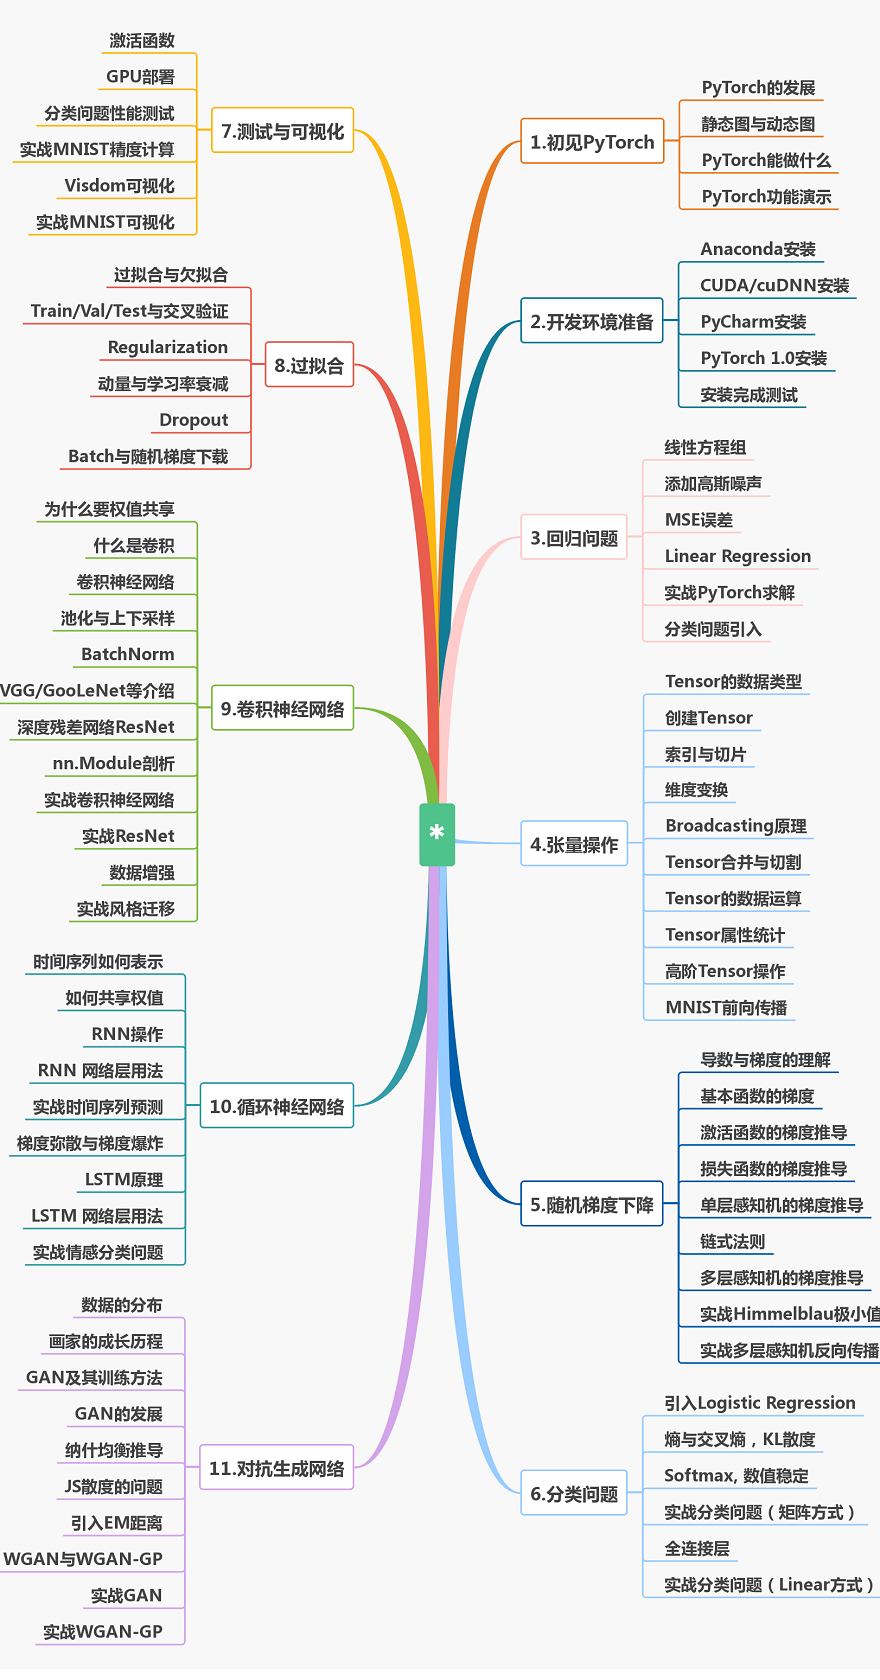
\includegraphics[width=0.9\textwidth]{PyTorch.png}
%  \caption{大纲图}
%\end{figure}
%\newpage 